\section{CHAPTER 5: PRODUCTION}

\subsection{Overview:}

The production process using Forbes Marshall components at Renaissance Apparel is 
a comprehensive sequence of operations that transforms raw knit fabric into finished dyed textile products. 
The system requires of a steam distribution system, boilers from Forbes Marshall. 
The facility operates 22 hours per day across three shifts, maintaining 
a production capacity of 30 tons per day (20 tons in Phase 1 and an additional 10 tons in Phase 2).


In the production section there is Dyeing, Knitting, Printing and Washing. There
was a soft flow machine for dyeing which produces 30 tons of products in
a day. There was a Slitting machine to make the round fabric into an
open form. Then there was a stenter machine for the dryer and heat
setting of the fabric. Thermic Oil used for stenter. There was a
Compacting machine as well for fabric shrinkage control. There were also
knitting machines producing 25 tons of products in a day. Fabric made in
a round shape here. This fabric is called Greig Fabric. The printing
machine was screen print type and 50 tons of products can be printed per
day. There were several washing machines whose capacity was 2000 per
day.\cite{knitting}

\subsection{Knitting Machine:}

The production journey begins with knitting, where yarns are interlaced to create fabric. 
These are on the second floor of the factory of the production line.
Mayer \& Cie Circular Knitting Machines are employed for this stage.

\begin{figure}[h!]
  \centering
  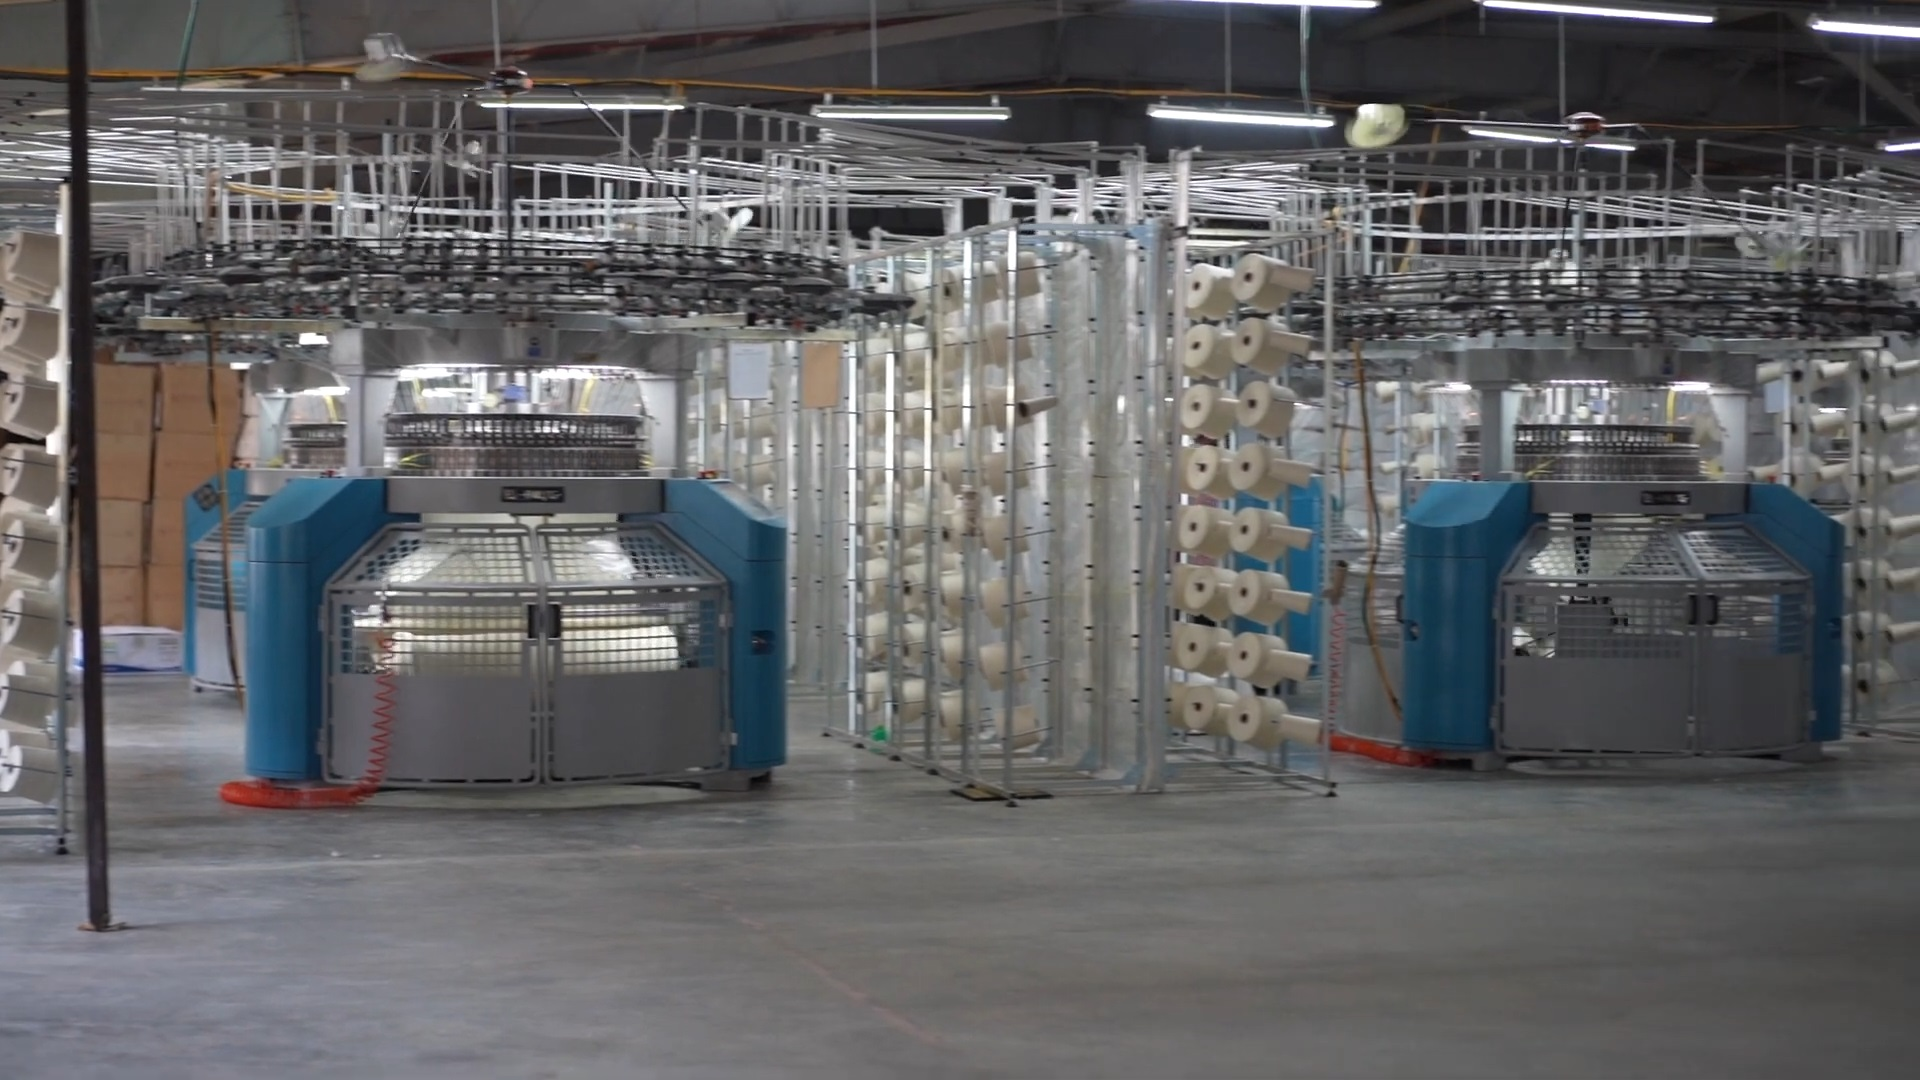
\includegraphics[width=0.8\linewidth]{figs/knitting.jpg}
  \caption{Knitting Machine}
  \label{fig:Knitting Machine}
\end{figure}

\begin{figure}[h!]
  \centering
  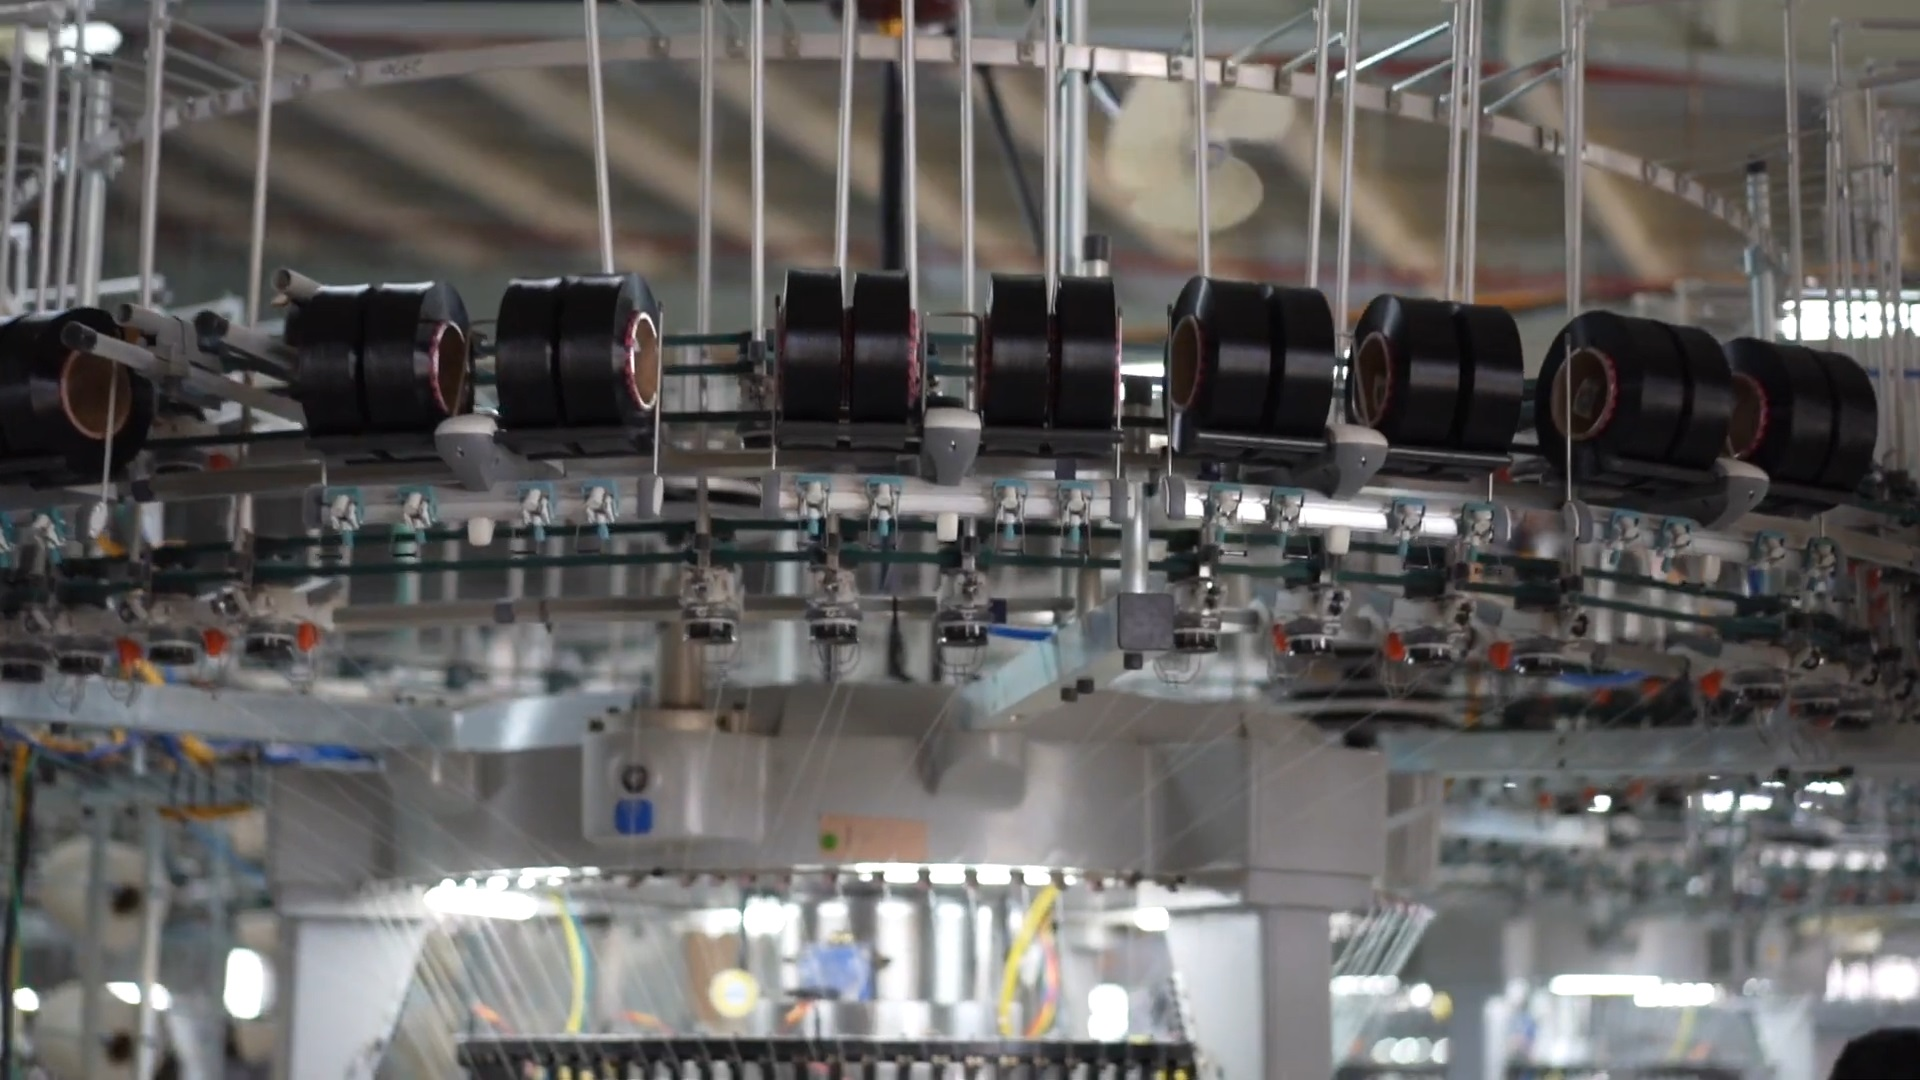
\includegraphics[width=0.8\linewidth]{figs/knitting_closeup.jpg}
  \caption{Knitting Machine Close Up}
  \label{fig:Knitting Machine Close Up}
\end{figure}

\subsubsection{Description:}
Knitting machines come in various types, including flatbed, circular,
and warp knitting machines. They consist of a needle bed, yarn feeders,
carriage or cam system, and controls for adjusting stitch size and
pattern.


\subsubsection{Functionality:}

\begin{enumerate}
\item
  Yarn Feeding: Yarn is fed into the machine from multiple feeders or
  cones, depending on the type of knitting machine.
\item
  Stitch Formation: Needles or hooks on the machine interlock the yarn
  to form loops or stitches, creating the fabric.
\item
  Fabric Formation: The carriage or cam system moves across the needle
  bed, manipulating the needles to form rows of stitches and build up
  the fabric.
\item
  Control: Knitting machines may have controls for adjusting stitch
  size, tension, and pattern to create different textures, designs, and
  structures.
\end{enumerate}

\subsubsection{Advantages:}

\begin{enumerate}
\item
  Versatility: Knitting machines can produce a wide range of fabrics,
  including jerseys, rib knits, and jacquards, with various textures,
  patterns, and thicknesses.
\item
  Efficiency: Knitting machines can achieve high production speeds,
  making them suitable for mass production of knitted garments,
  textiles, and accessories.
\item
  Customization: Knitting machines offer flexibility in design and
  customization, allowing for the creation of unique and personalized
  knitted products.
\end{enumerate}

\subsubsection{Disadvantages:}

\begin{enumerate}
\item
  Complexity: Operating and maintaining knitting machines require
  specialized skills and knowledge. Troubleshooting and repairing
  technical issues can be challenging.
\item
  Cost: Knitting machines can be expensive to purchase and maintain,
  especially advanced models with computerized controls and features.
\item
  Fabric Limitations: Knitting machines may have limitations in terms of
  fabric width, gauge, and complexity, restricting the types of fabrics
  and designs that can be produced.
\end{enumerate}

\subsection{Dyeing Machine:\cite{dyeing_machines}}

The greige fabric proceeds to the dyeing stage. 
Fongs Soft Flow Dyeing Machines are used to achieve gentle and uniform dyeing, 
capable of handling up to 30 tons of fabric daily.
Machines Used: Fongs Soft Flow Dyeing Machines (Model: THEN Airflow® Synergy 8).

It is a textile processing device used in the
dyeing of fabrics, primarily made from natural or synthetic fibers.

\begin{figure}[h!]
  \centering
  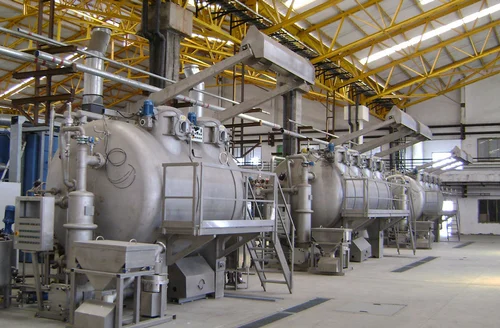
\includegraphics[width=0.8\linewidth]{figs/production/image1.png}
  \caption{Dyeing Machine}
  \label{fig:Dyeing Machine}
\end{figure}

\begin{figure}[h!]
  \centering
  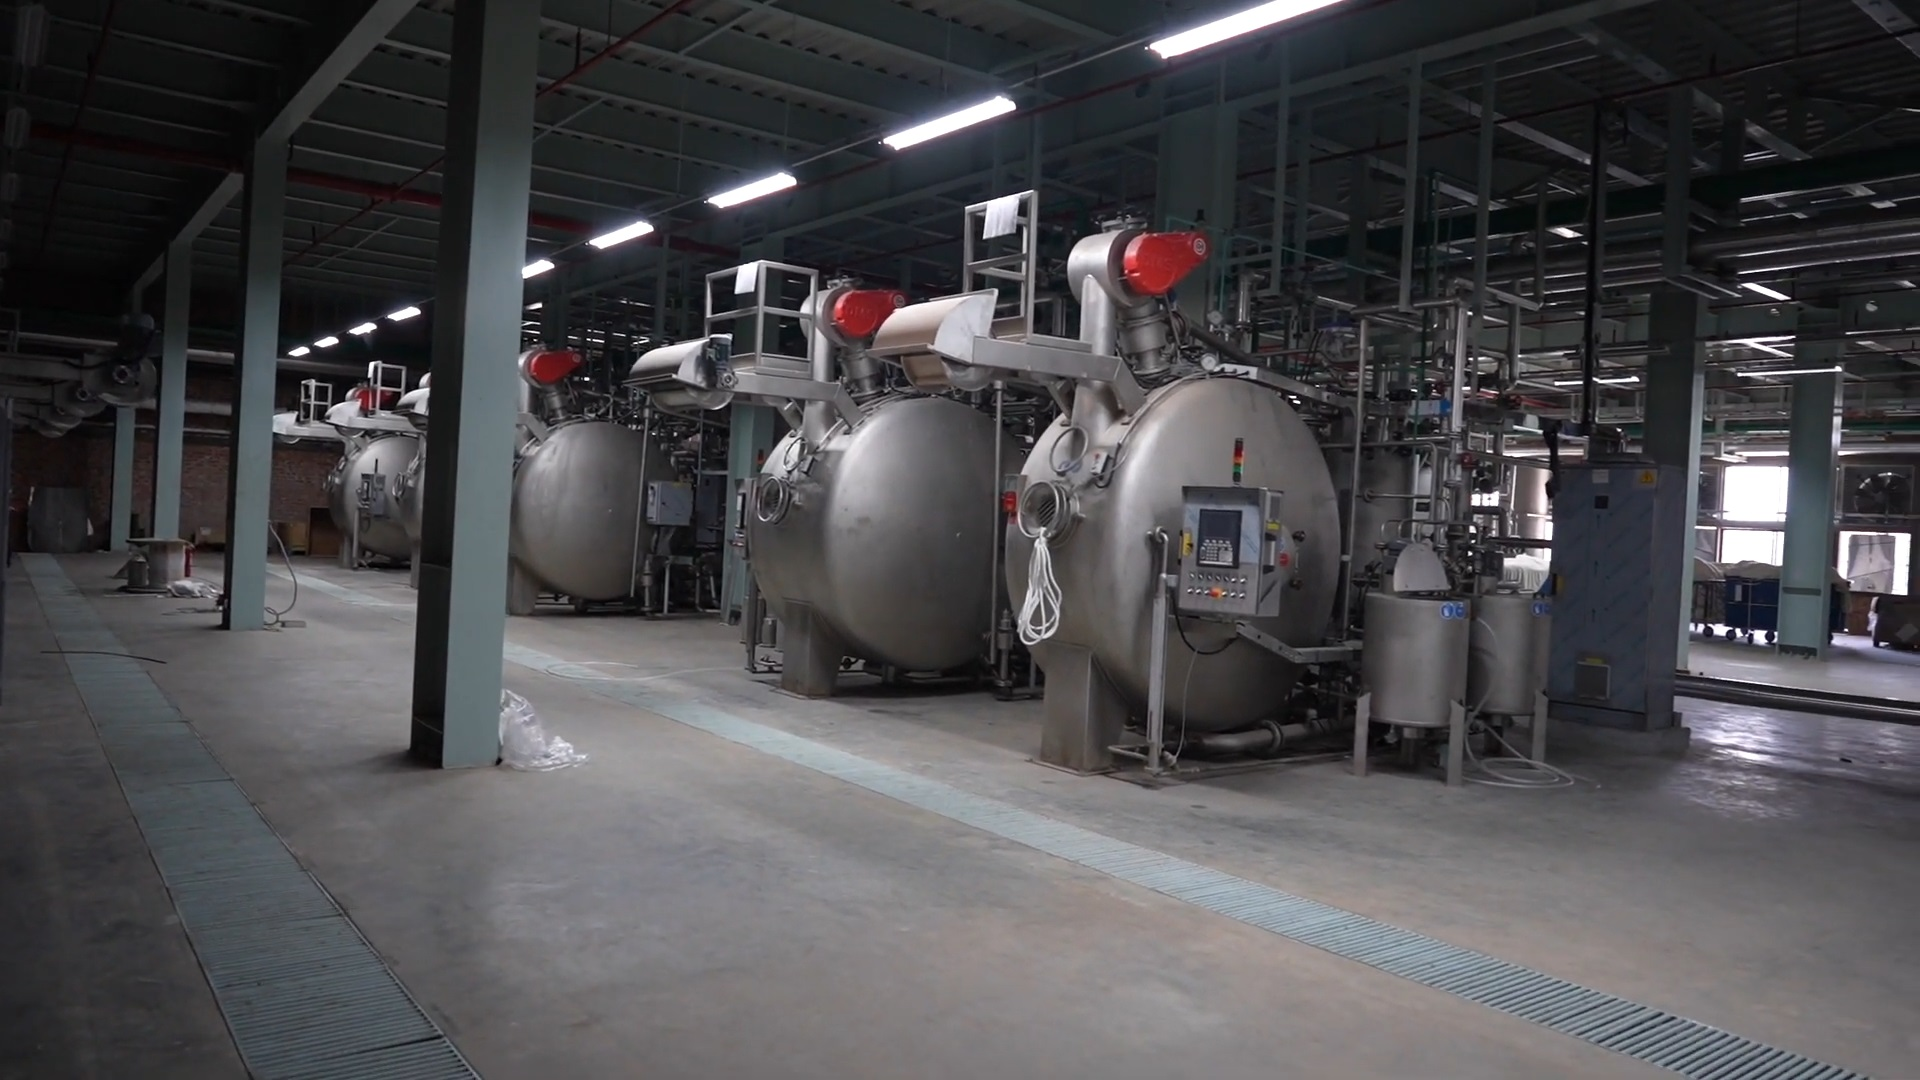
\includegraphics[width=0.8\linewidth]{figs/dyeing.jpg}
  \caption{Dyeing Machine 2}
  \label{fig:Dyeing Machine 2}
\end{figure}

\subsubsection{Description:}


These machines are designed to provide a gentle and uniform
dyeing process for delicate fabrics, ensuring minimal damage or
creasing. They operate by circulating a dye liquor through the fabric in
a controlled manner, allowing for even penetration of the dye solution
into the fibers.


\subsubsection{Functionality:}

\begin{enumerate}
\item
  Fabric Loading: Fabrics are loaded into the dyeing machine, either in
  loose form or on perforated rollers, to ensure even dye distribution.
\item
  Dye Liquor Circulation: The dye liquor, consisting of water, dye, and
  auxiliary chemicals, is circulated through the fabric using a
  combination of pumps, nozzles, and a specially designed flow system.
\item
  Temperature and Pressure Control: Soft flow dyeing machines maintain
  precise control over temperature and pressure parameters to ensure
  optimal dyeing conditions for different types of fabrics and dyes.
\item
  Dyeing Cycle: The dyeing process typically involves multiple cycles of
  dyeing, rinsing, and draining to achieve the desired color depth and
  uniformity.
\item
  Versatility: Soft flow dyeing machines are suitable for a wide range
  of fabrics, including cotton, polyester, wool, and blends, making them
  versatile for various textile applications.
\end{enumerate}

\subsection{Slitting Machine:}

After dyeing, the tubular fabric undergoes slitting to convert it into an open-width form using the Stanta Cut Slitting Machine.
It cuts large rolls or coils of material into narrower strips.



\begin{figure}[h!]
  \centering
  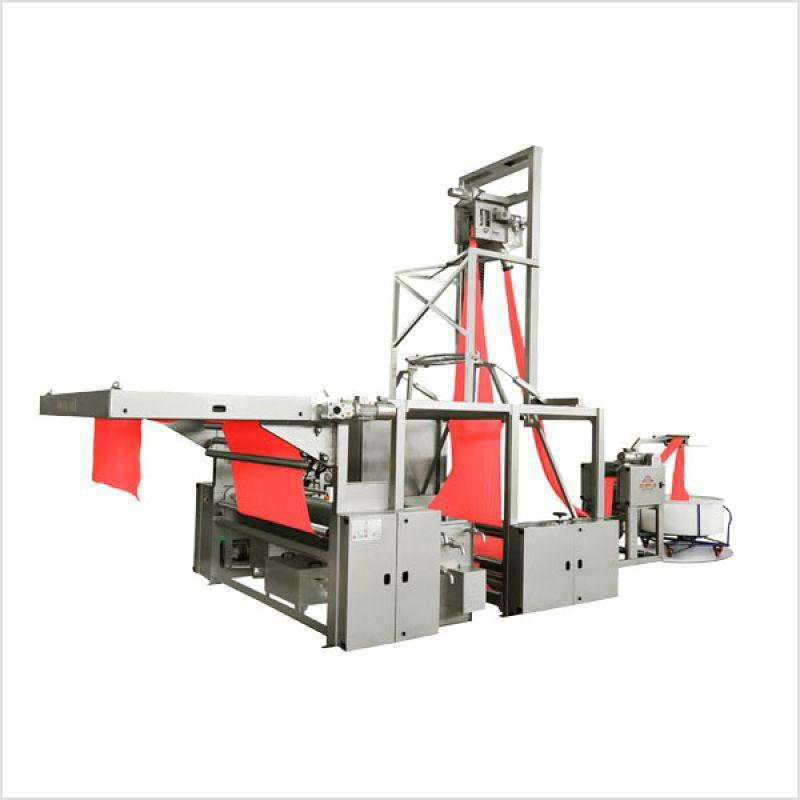
\includegraphics[width=0.8\linewidth]{figs/production/image2.jpg}
  \caption{Slitting Machine}
  \label{fig:Slitting Machine}
\end{figure}


\subsubsection{Description:}

Machine Used: Stanta Cut Slitting Machine.

Specifications:
Brand Name: Stanta Cut
Origin: Switzerland
Power Consumption: 10 kW
Speed: 60–70 m/min


\begin{enumerate}
\item
  Unwinder: Where the large roll or coil of material is loaded for
  processing.
\item
  Slitting knives or blades: These are used to cut the material into
  narrower strips.
\item
  Rewinder: Where the slit strips are rewound into smaller coils or
  spools.
\item
  Tension control system: Ensures proper tension is maintained on the
  material throughout the slitting process.
\item
  Control panel: Allows operators to adjust settings such as cutting
  width, speed, and tension.
\end{enumerate}

\subsubsection{Functionality:}

\begin{enumerate}
\item
  Material feeding: The roll or coil of material is loaded onto the
  unwinder and fed into the slitting machine.
\item
  Slitting: The material passes through the slitting knives or blades,
  which cut it into narrower strips. The number of blades and their
  spacing determine the width of the strips.
\item
  Rewinding: The slit strips are rewound onto individual cores or spools
  on the rewinder.
\item
  Quality control: Operators monitor the slitting process to ensure the
  strips are cut accurately and without defects.
\end{enumerate}


\subsection{Stenter Machine:\cite{stenter_machine}}

\begin{figure}[h!]
  \centering
  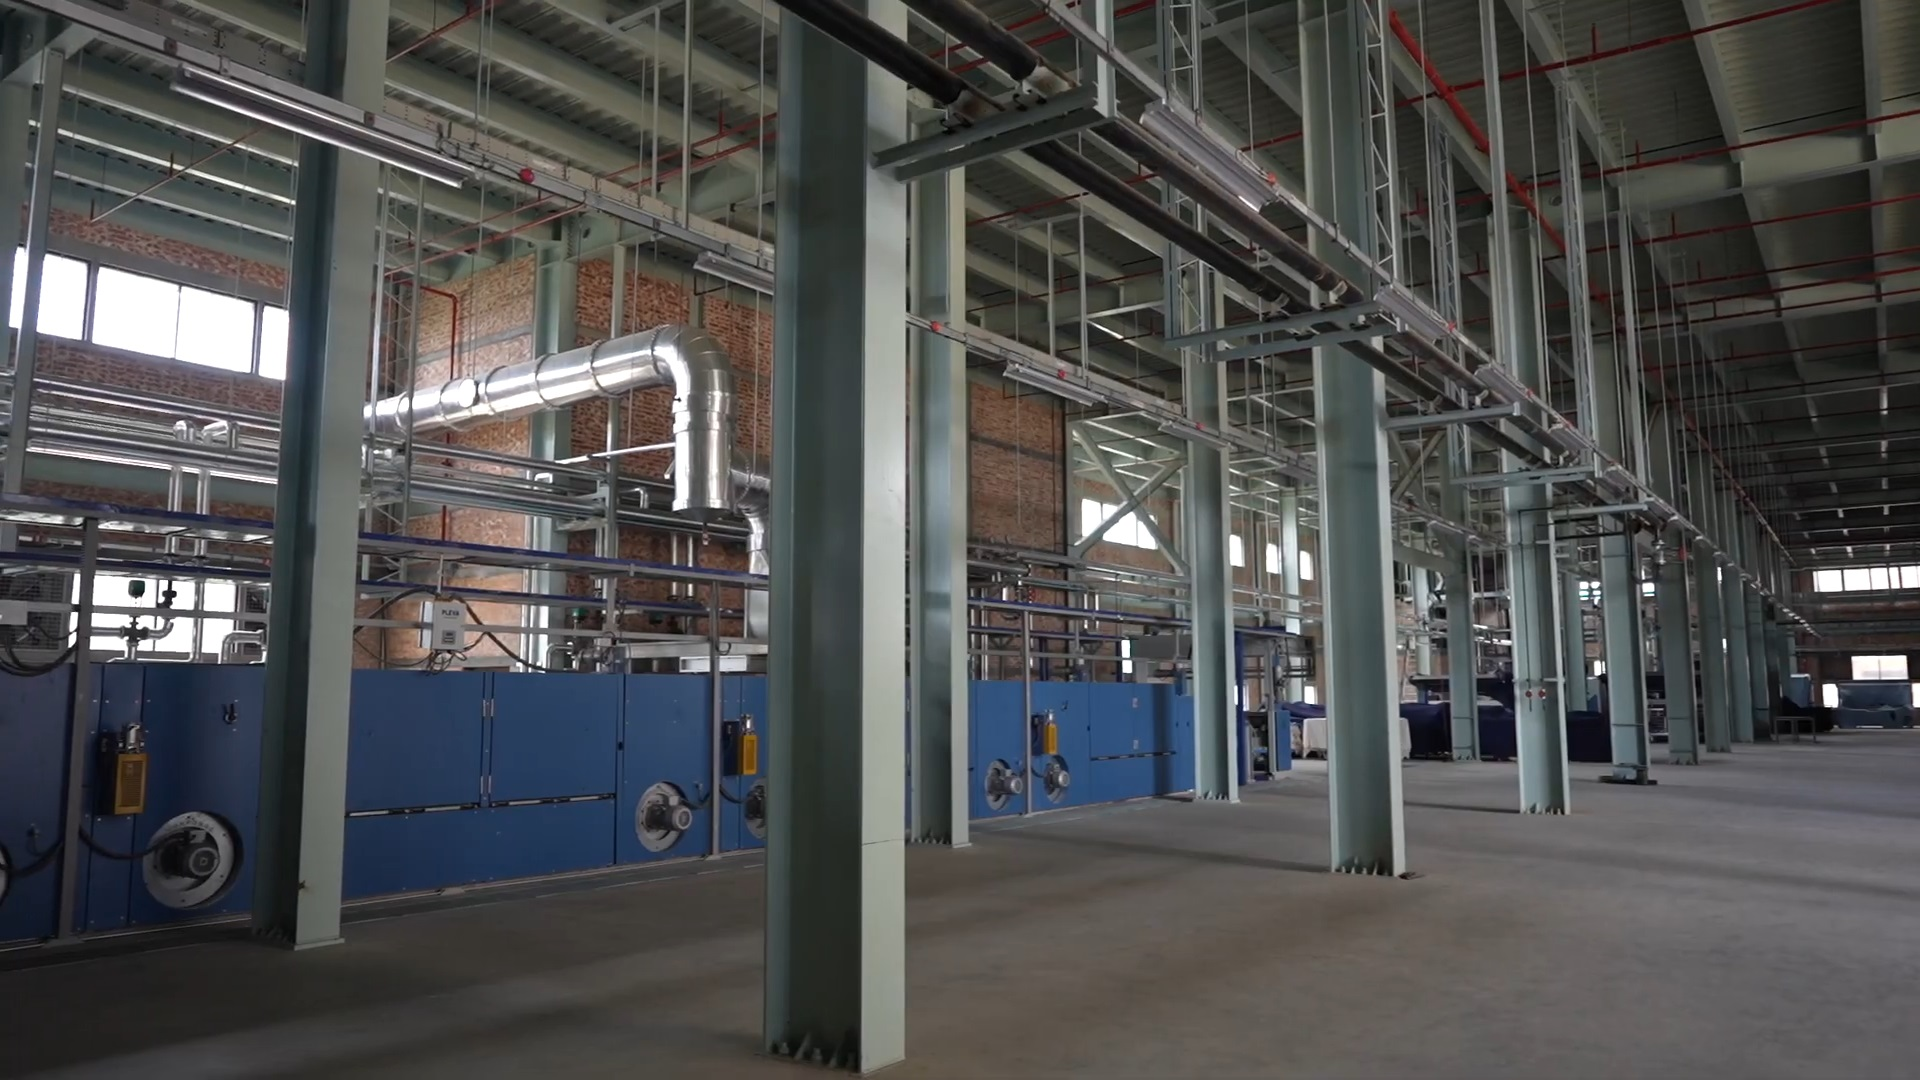
\includegraphics[width=0.8\linewidth]{figs/stenter.jpg}
  \caption{Stenter at Renaissance Apparel Ltd}
  \label{fig:stenter}
\end{figure}

\begin{figure}[h!]
  \centering
  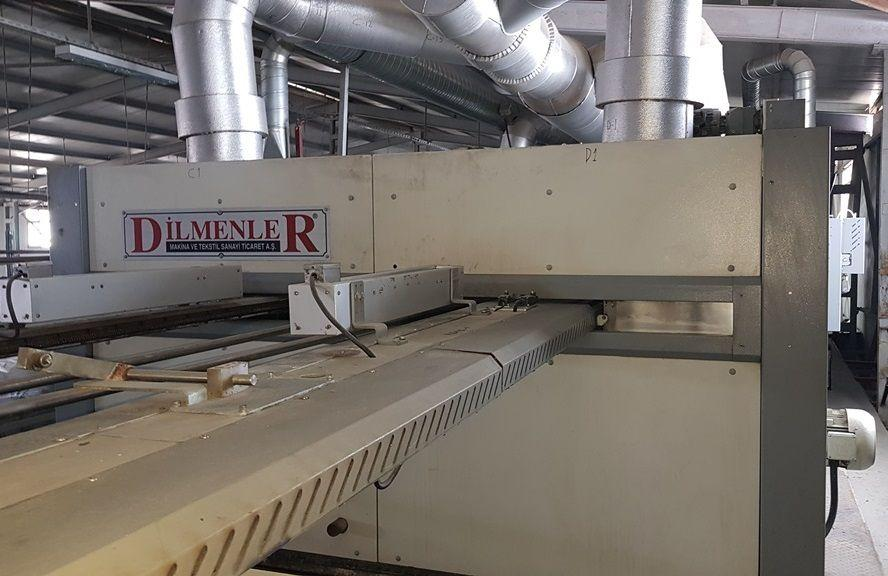
\includegraphics[width=0.8\linewidth]{figs/production/image3.jpg}
  \caption{Stenter Machine}
  \label{fig:Stenter Machine}
\end{figure}

The open-width fabric is thn subjected to stentering in the stentering machine, Dilmenler Stenter Machine, Model DLN-2100, 
involving drying and heat-setting to stabilize fabric dimensions.


\subsubsection{Description:}


A stenter machine typically consists of the following main components:


\begin{enumerate}
\item
  Entry and exit sections: Where the fabric enters and exits the
  machine.
\item
  Tentering chains: Continuous chains with clips or pins that hold the
  fabric edges taut and straight throughout the process.
\item
  Frame: Supports the tentering chains and other components of the
  machine.
\item
  Heating chambers: Where the fabric is subjected to heat to remove
  moisture and apply treatments or finishes.
\item
  Air circulation system: Ensures even distribution of heat and airflow
  across the fabric.
\end{enumerate}

\subsubsection{Functionality:}

\begin{enumerate}
\item
  Fabric feeding: The fabric is fed into the stenter machine from a roll
  or other source.
\item
  Tentering: The fabric is held taut and straight by the tentering
  chains, which stretch it to the desired width.
\item
  Heat treatment: The fabric passes through heating chambers, where it
  is subjected to controlled temperatures to remove moisture and apply
  treatments such as drying, curing, or coating.
\item
  Cooling: After heat treatment, the fabric may pass through cooling
  chambers to reduce its temperature and stabilize the applied
  treatments.
\item
  Finishing: Additional processes such as brushing, shearing, or
  calendering may be performed to achieve specific surface textures or
  finishes.
\item
  Fabric winding: The finished fabric is wound onto a roll or other
  suitable form for further processing or packaging.
\end{enumerate}



\subsection{Compacting Machine:}

The fabric moves to compacting, where shrinkage is reduced, and dimensional stability is enhanced.
It is particularly used for knitted fabrics.


\subsubsection{Description:}


Compacting machine used in Renaissance consisted of the following main
components:


\begin{enumerate}
\item
  Entry and exit sections: Where the fabric enters and exits the
  machine.
\end{enumerate}




\begin{figure}[h!]
  \centering
  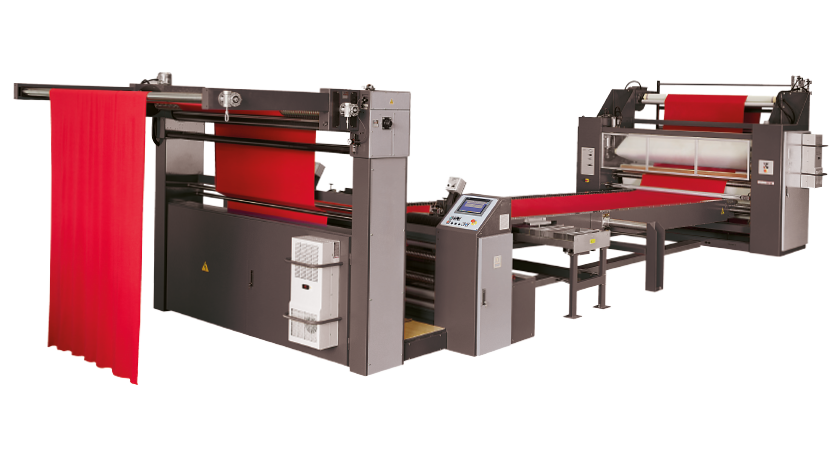
\includegraphics[width=0.8\linewidth]{figs/production/image4.png}
  \caption{Compacting Machine.}
  \label{fig:Compacting Machine.}
\end{figure}


\begin{enumerate}
\item
  Compacting rollers: These rollers compress the fabric, reducing its
  thickness and improving its dimensional stability.
\item
  Tension control system: Ensures proper tension is maintained on the
  fabric throughout the compacting process.
\item
  Heating system (optional): Some compacting machines may include a
  heating system to soften the fabric fibers, allowing for better
  compression.
\end{enumerate}

\subsubsection{Functionality:}

\begin{enumerate}
\item
  Fabric feeding: The fabric is fed into the compacting machine from a
  roll or other source.
\item
  Compression: As the fabric passes through the compacting rollers, it
  is subjected to pressure, which compresses the fibers and reduces the
  thickness of the fabric.
\item
  Heat treatment (optional): In some cases, the fabric may be subjected
  to heat during the compacting process to soften the fibers and enhance
  the compression effect.
\item
  Cooling: After compression, the fabric may pass through cooling
  chambers to reduce its temperature and stabilize its properties.
\item
  Fabric winding: The compacted fabric is wound onto a roll or other
  suitable form for further processing or packaging.
\end{enumerate}


\subsection{Printing Machine:} 
The treated fabric undergoes printing using the Zimmer Rotary Screen Printing Machine (Model: Magnoprint), capable of processing up to 50 tons of fabric daily.

\begin{figure}[h!]
  \centering
  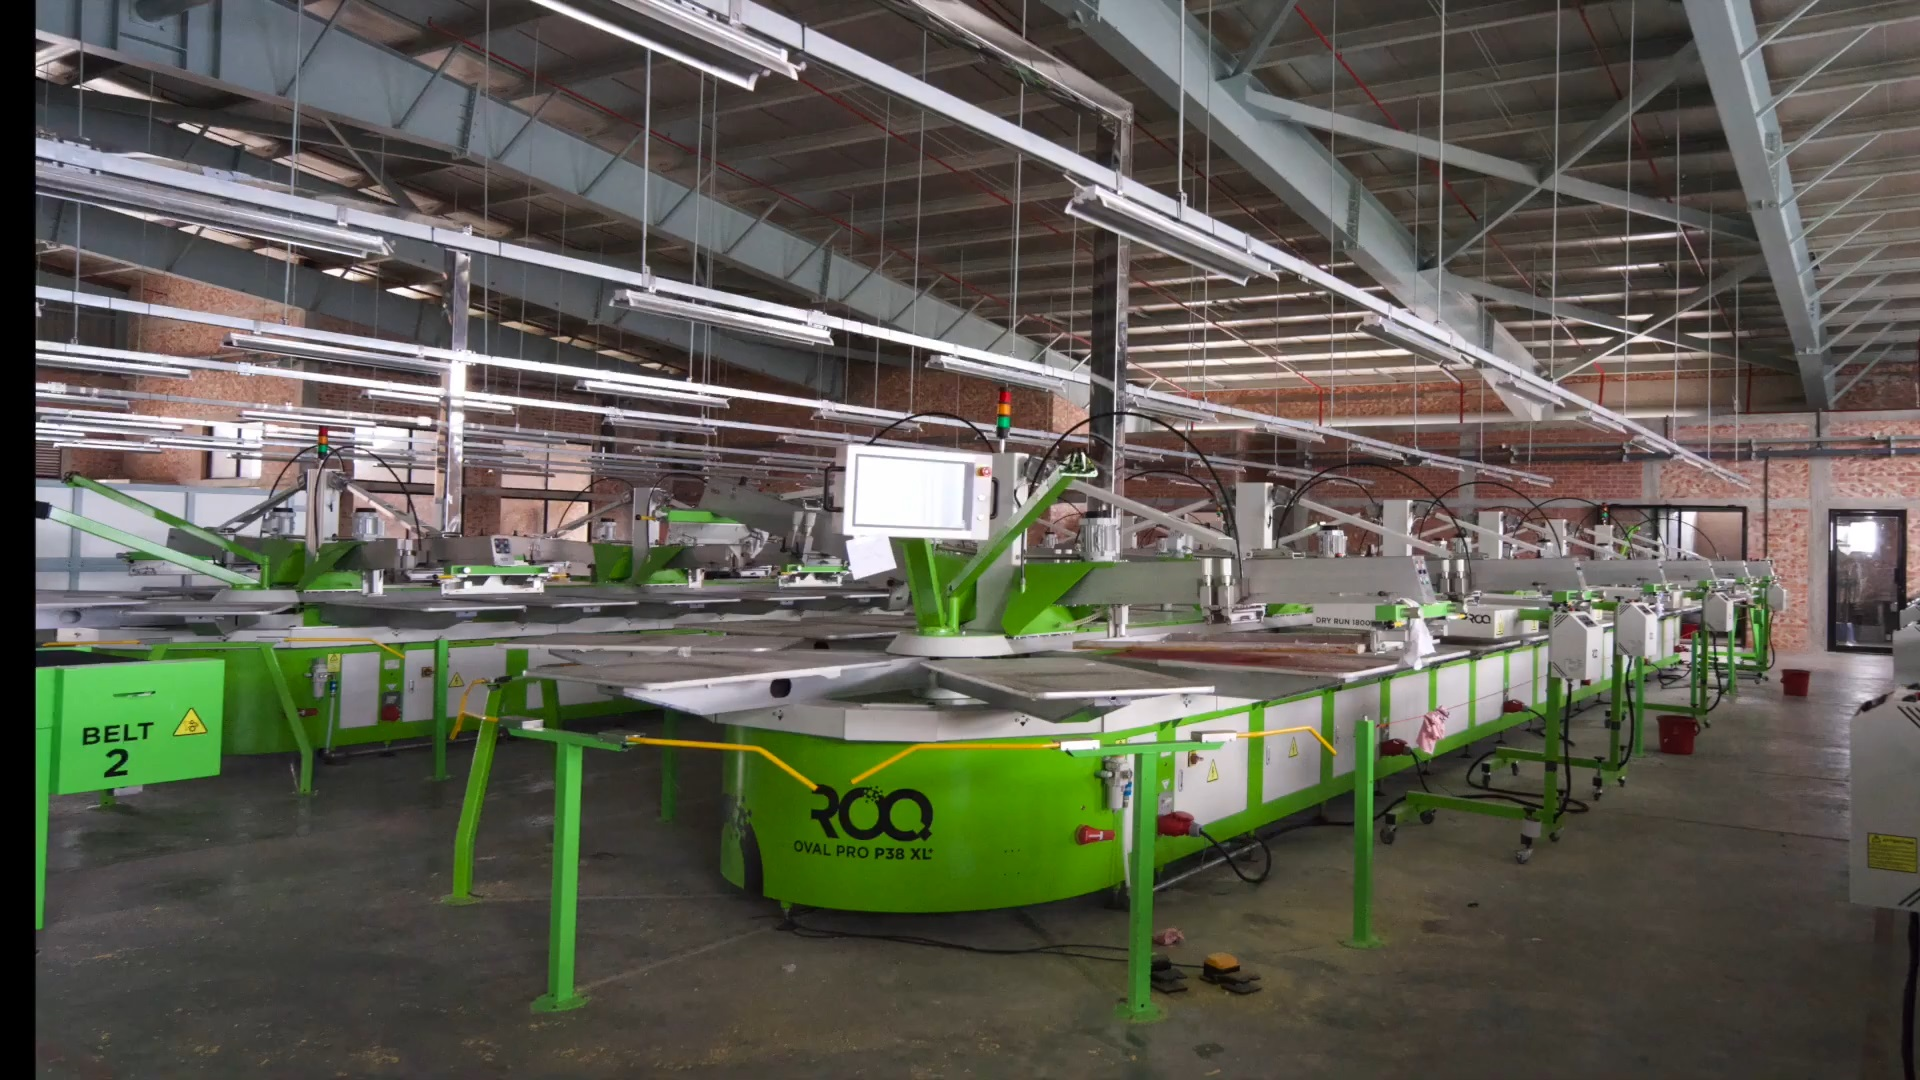
\includegraphics[width=0.8\linewidth]{figs/placement_printing.jpg}
  \caption{Printing Machine}
  \label{fig:Printing Machine}
\end{figure}

\subsubsection{Description:}


The machines in Renaissance consists of the following main
components:


\begin{enumerate}
\item
  Screen frame: A frame made of wood, aluminum, or steel, with a
  stretched mesh screen tightly attached.
\item
  Squeegee: A rubber or plastic blade used to push ink through the mesh
  screen onto the substrate.
\item
  Printing bed: The surface where the substrate is placed for printing.
\item
  Registration system: Guides or stops to ensure accurate alignment of
  the substrate for multiple-color printing.
\item
  Ink reservoir: A container for holding the printing ink, typically
  located above the screen frame.
\end{enumerate}

\subsubsection{Specifications:}

Printing Width: Up to 3200 mm
Number of Colors: Up to 12
Speed: Up to 120 m/min


\subsubsection{Functionality:}

\begin{enumerate}
\item
  Preparation: The design to be printed is first transferred onto a
  stencil or mesh screen using a photographic process or manually
  applied emulsion.
\item
  Setup: The substrate is placed onto the printing bed, and the screen
  frame is positioned over it.
\item
  Ink application: Ink is poured onto the screen frame, and a squeegee
  is used to spread the ink evenly across the screen.
\item
  Printing: The squeegee is then pulled across the screen, forcing the
  ink through the mesh and onto the substrate, creating the desired
  design or pattern.
\item
  Curing: After printing, the substrate may pass through a curing or
  drying process, typically involving heat or UV light, to set the ink
  and ensure durability.
\end{enumerate}


\subsection{Washing Machine:}
\begin{figure}[h!]
  \centering
  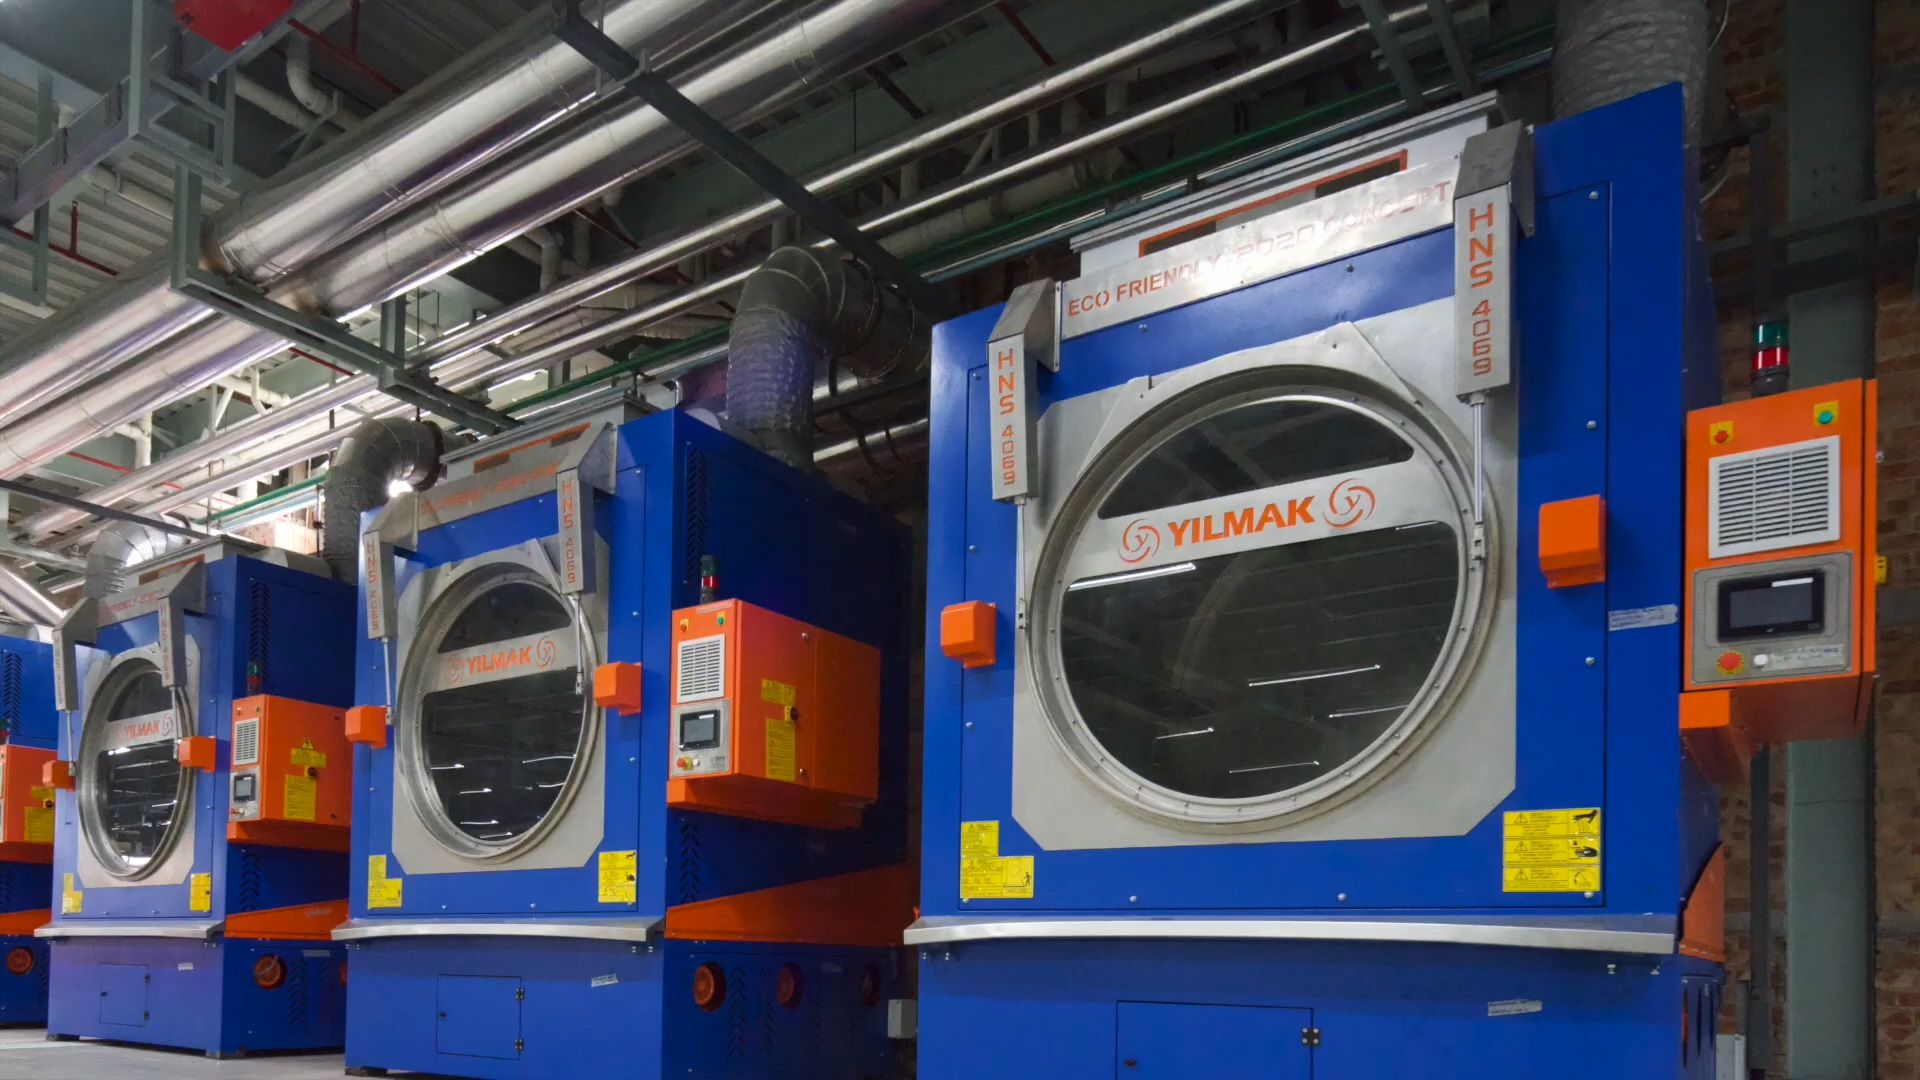
\includegraphics[width=0.8\linewidth]{figs/washing.jpg}
  \caption{Washing at Renaissance Apparel Ltd}
  \label{fig:washing}
\end{figure}

A washing machine is a textile processing device used to clean and finish fabrics after dyeing, printing, or other treatments.

Machine Used: Yilmak Washing Machine (Model: HNS 405)

\subsubsection{Specifications:}
Load Capacity: 500 kg per batch
Steam Utilization:
Steam Pressure: 8.5 - 10.5 BarG
Steam heats the wash water to temperatures up to 98°C for efficient cleaning.
